\documentclass[conference]{IEEEtran}

\usepackage{cite}
\usepackage{amsmath,amssymb,amsfonts}
\usepackage{algorithmic}
\usepackage{textcomp}
\usepackage{xcolor}
\usepackage{tikz}

\begin{document}

\title{
    EECS 126 Project Proposal \\
    {\footnotesize An Implementation of a MCMC Approach for Markov Random Field Super-resolution Image Reconstruction}
}

\author{
    \IEEEauthorblockN{Chong, Raymond}
    \and
    \IEEEauthorblockN{Chui, Tin Hang}
    \and
    \IEEEauthorblockN{Meng, Fanyu}
    \and
    \IEEEauthorblockN{Qin, Zipeng}
}

\maketitle

%\begin{abstract}
%This document is a model and instructions for \LaTeX.
%This and the IEEEtran.cls file define the components of your paper [title, text, heads, etc.]. *CRITICAL: Do Not Use Symbols, Special Characters, Footnotes, 
%or Math in Paper Title or Abstract.
%\end{abstract}
%
%\begin{IEEEkeywords}
%component, formatting, style, styling, insert
%\end{IEEEkeywords}

\section{Introduction}
This research aims to use the Markov Chain Monte-Carlo (MCMC) sampling method to achieve super-resolution image reconstruction. The goal of super-resolution image reconstruction is to construct a higher resolution image given one, potentially blurred and slighted tweaked, with lower resolution. This could be very useful for enhancing images or being a preliminary step for other image processing such as image recognition. Similar to Markov-chain modeled text generation, as shown in Fig. \ref{img:mrf_eg}, image generation can be considered as a 2-dimensional Markov random field (MRF), where each pixel is conditionally independent from all other pixels except its neighbors: 
\begin{align}
    p(X_{ij}|X) = p\big(X_{ij}|\{X_{kl}~| kl \text{ is a neighbor of } ij\}\big)
    \label{eq:pixel_dist}
\end{align}
where $X$ is an image, and $X_{ij}$ is the pixel in the $i$-th row and $j$-th column of $X$. This model is considered useful for super-resolution problems. \cite{tian2012bayesian} Similar to linear Markov chains, we can train a Bayesian distribution of a pixel conditioned on its neighbors, and use Gibs' sampling to generate the result. \cite{tian2005mcmc}

\begin{figure}[h]
\centering
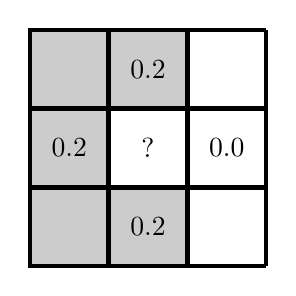
\begin{tikzpicture}
    \draw [ultra thick, draw=black, fill=black!20!white] 
    (0,0) grid (3,3)
    (1,2) rectangle (2,3)
    (0,0) rectangle (1,3)
    (1,0) rectangle (2,1);
    \node at (1.5,0.5) {0.2};
    \node at (0.5,1.5) {0.2};
    \node at (1.5,2.5) {0.2};
    \node at (2.5,1.5) {0.0};
    \node at (1.5,1.5) {?};
\end{tikzpicture}
\caption{An example image where the number in the grid symbolize the brightness of the pixel. Empirically, assuming we only consider the 1-neighbors and we have enough edge-like training samples, the pixel at ? should have a higher probability to be 0.2.}
\label{img:mrf_eg}
\end{figure}

\section{Methods}
We will try to reconstruct a higher-resolution stylized images such as image of texts or anime-style images using the method based on Jing Tian and Kai-Kuang Ma's research ``A mcmc approach for bayesian super-resolution image reconstruction'' \cite{tian2005mcmc}. We assume that the images conform to a Gaussian MRF prior:
\begin{align}
    p(\mathbf{X}) 
    = \frac{1}{(2\pi)^{M/2} |\mathbf{C}^{-1}|^{1/2}} 
        \exp\left\{-\frac 1 2 \lambda \mathbf{X}^{T}\mathbf{CX}\right\}
    \label{eq:gmrf}
\end{align}
where $X$ is the original image, $\lambda$ is the positive scaling parameter and $\mathbf C$ is the incidence matrix:
\begin{align}
    \mathbf{C}_{ij} = \begin{cases}
        \gamma, &\text{i = j} \\
        -1, &\text{if }i\text{ and }j\text{are adjacent in }\gamma\text{-neighborhood} \\
        0, &\text{otherwise} 
    \end{cases}
    \label{eq:c_mat}
\end{align}
However, to compensate for small noise pixels and to capture the style of the original image, we will apply a convolution layer and a max pooling layer before we train the model. The generated image will be in the same resolution with the image after the convolution and pooling. We will train the conditional distributions in \eqref{eq:pixel_dist}, and use Gibs' sampling to sample from the distribution $p(\mathbf{X}|\mathbf{Y})$ and the MAP estimate for $\mathbf{X}$ is given by
\begin{align}
    \hat{\mathbf{X}} = \mathbb{E}\big[p(\mathbf{X}|\mathbf{Y})\big]
    \label{eq:map_est}
\end{align}
where $\mathbf{Y}$ is the low resolution image.

\bibliographystyle{IEEEtran}
\bibliography{project_proposal}

\end{document}
